%%%% ijcai18.tex

\typeout{IJCAI-18 Instructions for Authors}

% \setcounter{secnumdepth}{5}

% These are the instructions for authors for IJCAI-18.
% They are the same as the ones for IJCAI-11 with superficical wording
%   changes only.
\documentclass{article}
\pdfpagewidth=8.5in
\pdfpageheight=11in
% The file ijcai18.sty is the style file for IJCAI-18 (same as ijcai08.sty).
\usepackage{ijcai18}

% Use the postscript times font!
\usepackage{times}
\usepackage{xcolor}
\usepackage{soul}
\usepackage[utf8]{inputenc}
\usepackage[small]{caption}

% the following package is optional:
%\usepackage{latexsym} 

\usepackage{graphicx}
\graphicspath{ {./} }

\usepackage{hyperref}

\hypersetup{
    colorlinks=true,
    linkcolor=blue,
    filecolor=magenta,      
    urlcolor=cyan
}

\title{Limit Texas Hold'em Poker Agent built using an Adversarial Approach - Team \#02}

% Multiple author syntax (remove the single-author syntax above and the \iffalse ... \fi here)

\author{
Amrut Prabhu,
Archana Pradeep,
Lim Jun Hao,
Shreyas Kuthanoor Prakash,
Zhong Zheng Xin
\\ 
National University of Singapore\\
A0162655B, A0162694W, A0147944U, A0177064B,A0160045U 
}

% If your authors do not fit in the default space, you can increase it 
% by uncommenting the following (adjust the "2.5in" size to make it fit
% properly)
% \setlength\titlebox{2.5in}

\begin{document}

\maketitle

\section{Introduction}

Limit Texas Hold’em is a simplified version of the poker game. When playing in a game of poker,  the money always flows between the players, and there is no additional money coming into or going out of the game. It remains a fixed amount. Also, it is impossible to know with full certainty, the cards that your opponents have as well as what the community cards on the table will be. Thus, poker is a zero-sum game with an element of uncertainty. 

When using a Poker bot, It is not computationally feasible to look at all possible states of the poker game before making a decision about what action \footnote{Possible actions are: raise, call and fold} to take. A smarter approach that uses intuition (i.e. heuristics) to make better decisions is required. Hence, the aim of this project is to design and implement such an agent, that can optimally play a 2-player game of Limit Texas Hold’em Poker.

\subsection{Our Approach} 

This report discusses an Adversarial strategy that is designed to make optimal decisions in 2-player Limit Texas Hold’em poker (hereafter referred to as poker) games. This makes sense intuitively because, as described above, poker is a zero-sum game in which you, the player, have an adversary, your opponent, who is trying to win your money and vice versa.

\begin{itemize}
    \item {\bf Heuristics}:
        Before deciding on a strategy, we looked into generating heuristics that are simple and effective. Though we use many implicit heuristics, the 3 heuristic functions that we use - Win rate, Effective Hand Strength, and Amount in Pot - are described in Section 2.1.
    \item {\bf MiniMax Search Tree}:
        The Adversarial strategy used by our agent is implemented as a MiniMax search tree that also uses alpha beta pruning, as described in Section 2.2. The utility function used at the terminal nodes is a weighted combination of the 3 heuristic functions. 
    \item {\bf Genetic Algorithm to determine weights}:
        As mentioned above, each of the 3 heuristics is assigned a weight, which is used when determining the utility function of a terminal state. The optimal values of these weights is found using the genetic algorithm described in Section 3. Basically, the best "parents" in each generation of players are used for creating a child parent.
\end{itemize}

\section{Adversarial Search}

As mentioned in Section 1, Poker is a zero sum game. Hence, it can intuitively be modelled as a game with an adversarial opponent. But first, we need to define the heuristics that are able to capture the state of the game, and help our agent make an optimal decision to achieve a Nash equilibrium.

\subsection{Heuristics}
The poker agent makes use of a linear weighted sum of the heuristics as the heuristic function for a given state. Given a state and a set of valid actions, the agent computes the heuristic function values for all the next set of actions the agent can make and then greedily picks the next state which has the maximum/minimum heuristic value depending on whether it is a small blind or big blind.
We have 3 explicit heursitics, but many implicit ones.
% {\tt https://pdfs.semanticscholar.org/1071/c0f275e5412825d46558e35267a8e03d2b2c.pdf}

\subsubsection{Win Rate}

The win rate for the player given the current state is the {\bf most important heuristic} for optimal decision making.

\textbf{Pre-flop:} There are a small number of possible starting hole card combinations and the win rate for every hole card combination can easily be pre-determined and hard coded. We’ve obtained data from \href{https://www.cs.indiana.edu/~kapadia/nofoldem/2_wins.stats}{here} which provides the win rate for every hole card combination [Anu Kapadia (n.d.)]. The data is generated by playing 4 billion simulated games in a 1v1 fashion. The \texttt{\detokenize{eval_pre_flop(hole_cards)}} function will simply return the win rate from the hard coded data.

\textbf{A naive hand evaluator:} This game is played in a fixed 1v1 fashion and thus we can easily get an accurate win rate by considering the probability of the opponent getting a hand better than ours. By first determining the bot’s best hand, we simply need to calculate the odds of the opponent getting a better hand. For example, the bot has a flush with an Ace high (the highest card in his hole cards that is part of the flush) which is the highest possible flush. Hence, to get the win rate of the bot’s current hand, we check if the community cards can from any stronger hands (full house, four of a kind, straight flush, royal flush) and determine the odds of that.
This method is easily doable for the river street and will compute very quickly. However this is a problem in the flop and turn streets as there are more community cards to draw and to get the win rate for the current state, it has to simulate the win rate of every possible community card to be drawn and average it. This can be computationally intensive especially for the flop street where it needs to calculate up to 48C2=1,128 different scenarios.

The issue can be solved using a Look-Up Table (LUT) by pre-computing all possible states, ever 7-card combination (2 hole cards and 5 community cards), 6-card combination and 5-card combination. However a new issue arises, 7-card combinations will result in 52C2*50C5=2,809,475,760 states and will be about 10GB in size. The states may be reduced with the fact that some states are identical (since suits are treated equally); LUT size can be reduced but not enough. For 6-card combinations and 5-card combinations, there are significantly much less states (305,377,800 and 25,989,600 respectively before reductions) and these will result in a LUT size that is reasonable (under 300MB in total with compression).

Since calculating a win rate for one state is fast enough to be done real-time, win rate during the river street will be computed in real-time while win rates for flop and turn streets will be provided by the LUTs.

\subsubsection{Effective Hand Strength based on Opponent Model}

The Effective hand strength heuristic provides an accurate assessment of our agent’s winning chances by using an opponent model and the present game state. This evaluation has two stages- pre-flop and post-flop evaluation because the community cards get opened in stages. The pre-flop evaluation calculates the hand strength of our private cards while the post-flop evaluation takes into account both the hand strength and the potential of our private cards. Here, the hand strength assesses how strong our hand is while the hand potential is the probability of our hand becoming the strongest hand when future community cards are dealt. 

For a set of two cards, there are 169 distinct hand types (13 paired hands). For each of these hand types, a statistical measure of the approximate return of our investment is calculated and stored as an array of weights. This array of \href{http://poker.cs.ualberta.ca/publications/papp.msc.pdf}{weights} thus serves as a distribution of the expected value our cards gain [Denis Richard Papp, 1998]. 

{\bf Hand Strength}: The Hand Strength calculation is done on the flop, turn and river and provides an estimate of the probability that our hand is the strongest hand. With the set of weights defined earlier, we calculate the strength of our cards relative to what other players may hold. By obtaining a percentile ranking of our hand using the weighted sum, the strength becomes the measure of the hands we are ahead divided by the total possible hands

{\bf Hand Potential}: The head potential is the probability that our hand improves as more community cards get opened. For example, consider the cards 3 of Hearts and 6 of Clubs. These two cards have a very weak hand strength. Suppose the community cards which open up on the flop are 4 of Hearts, 5 of Hearts and 10 of Hearts. Now our weak cards have tremendous potential for improvement. A single Hearts card or 2 or 7 can give us a flush or a straight. Thus, there is a high possibility for our hand to improve. 

We thus define positive potential as the probability of getting a better hand when we are behind. This can be evaluated by looking at the combinations of cards which result in us being ahead when we were behind. In order to obtain this value, we look-ahead to possible turn and river cards which might turn up.

{\bf Effective Hand Strength}: The Effective Hand Strength (EHS) represents the strength of our hand in the current game state. It is an estimation of the probability that our hand is leading or will improve to the strongest hand after the community cards are dealt. Thus, it a combination of both Hand Strength and Hand Potential and is calculated as follows:

$EHS = Hand\_Strength + (1 - Hand\_Strength) * Positive\_Potential$

Though the Effective Hand Strength heuristic is quite effective in assessing the strength of our hand, it is quite exhaustive computationally and takes a large time to provide accurate values, which resulted in Timeout exceptions during the early stages. Thus, we reduced the number of simulations needed for obtaining the weighted sum by taking random values in order to improve on the time taken. 

\subsubsection{Amount in Pot}

The Amount in Pot heuristic provides an assessment of the amount in play and can guide the agent's action along with the other heuristics. For a weak hand, our agent might find to better to fold at an early stage in order to reduce the amount in the pot, effectively cutting down his losses. Similarly, with a very strong hand, the agent might raise more to increase the pot amount. 

\subsection{Strategy}
Minimax is a decision-making algorithm , usually used in turn-based two player games. The goal of the algorithm is to find the next optimal move from its current position on the game tree.

The decision is made using a MiniMax tree with alpha-beta pruning. MiniMax is an adversarial search algorithm that recursively calls two functions $Max$ and $Min$ to determine the next move that the player should take. In the case of our poker agent that means choosing between fold, call or raise depending if these are valid actions from the previous move. We do a depth-limited MiniMax by going to a certain depth in the game tree and then moving upwards while performing MiniMax.  

The pre-flop stage is pre-computed as the decision tree is exhaustive while the post-flop stage is when the MiniMax strategy is used. The MiniMax function has two terminal tests which determines where it should start computing the weighted heuristics. One is whether the predetermined max depth has been reached and the other is whether the agent is in the last round of the game. Else the the MiniMax traverses the tree further and updated Alpha (Max strategy) and Beta (Min strategy) until it determines the next best action to take. 

In the case of the MiniMax tree, how the evaluation of the heuristics is done is very important. As mentioned in the above sections, the 3 heuristics whose sum is taken to evaluate the next action are opponent behaviour, strength of agent’s hand and amount in pot. These heuristics are given appropriate weights using the genetic algorithm and this helps the agent come up with the next best decision to take.

\section{Determining Heuristic Weights}

In our approach, we used a genetic algorithm to determine the optimal weights for the linear combination of the 3 heuristics. 

A {\bf genetic algorithm} is a method that is used for solving optimization problems. In the case of building our Poker agent, the genetic algorithm is used to determine the best values for the weights of our heuristic functions, such that our agent plays as optimally as possible.

Genetic algorithms can be thought of as search heuristics that are based on Charles Darwin’s theory of natural selection, which is the process that drives biological evolution. In the process, the fittest \footnote{Here, fitness is a measure of how well the agent is able to compete with other agents in the generation}  entities of each generation of the population are selected, and are made to reproduce an offspring for the next generation. When the parents have a better fitness score, their offspring will be better than them, and will have a higher likelihood of surviving. At the same time, the not-so-fit entities are killed off and do not contribute to the next generation. The reason for doing so is to increase the diversity of entities seen,  and to ensure that the best characteristics of one generation are passed down to the next, which in turn passes it down, and so on. This process is done iteratively until it converges to a generation that has entities that have very good fitness scores. 

More concretely, there are 4 steps in the genetic algorithm that was used for training the heuristic weights of our poker agent:

\begin{enumerate}
\item{{\bf Generate an initial population}

    The first step is to spawn instances of our player (agent) to get a starting population of players. Each player instance varies slightly, as they have a different set of assigned heuristic weights. These weights are obtained by using a random real-valued number (within a certain range), and adding or subtracting it from the default heuristic weights that is defined.
    
    Here, there are a few variables that need to be set. These are the hyperparameters of our genetic algorithm. In this step, we have seen 3, namely, population size (number of agents), default heuristic weights, and maximum possible offset from these default weights. These hyperparameters are discussed in more detail in the next subsection, and in the Discussion section.
}
\item{{\bf Calculate fitnesses}

    After having a population to work with, the fitness of each player in the population relative to the other players is computed. In order to do so, the players are made to play a game of poker against each other. The amount in the player’s stack is used as the fitness measure for that generation (or epoch or iteration). In simple terms, the player who wins the game is regarded to be fitter than the player that lost.
    
    In our implementation, in an epoch, the fitness measure of a player plays is determined from its results in 1v1 games of poker against two randomly selected players. This fitness measure is then used to update the player’s weights.
}
\item{{\bf Select parents for next generation}

    The fitness measures of all the players in the population is used to generate a probability distribution. This distribution determines the likelihood of a player being selected as a parent for the players of the next generation.

    The parents for our next generation of players is selected randomly from the probability distribution of the current generation. The number of parents selected is half that of the population size.
}
\item{{\bf Reproduce players for next generation}

    The final step of the process is determining the players that will be present in the next generation of the population. The players for the next generation can be reproduced by:

    \begin{itemize}
        \item{
            {\bf Mutations}: This involves ... This is done to maintain diversity within the population and prevent premature convergence.
        }
        \item{
            {\bf Elitism}: This creates a child that is identical to the parent. So, the parent player will be reproduced as-is in the next generation.
        }
        \item{
            {\bf Crossover}: For each pair of parents to be mated, a crossover point is chosen at random from within the genes. The weights (or {\textit genes}) of the first parent from before the crossover point become part of the child's weights. The remaining weights are selected from the second parent. This is shown in the Fig. \ref{fig:crossover}. 
    
             \begin{figure}[!t]
            	\centering
            	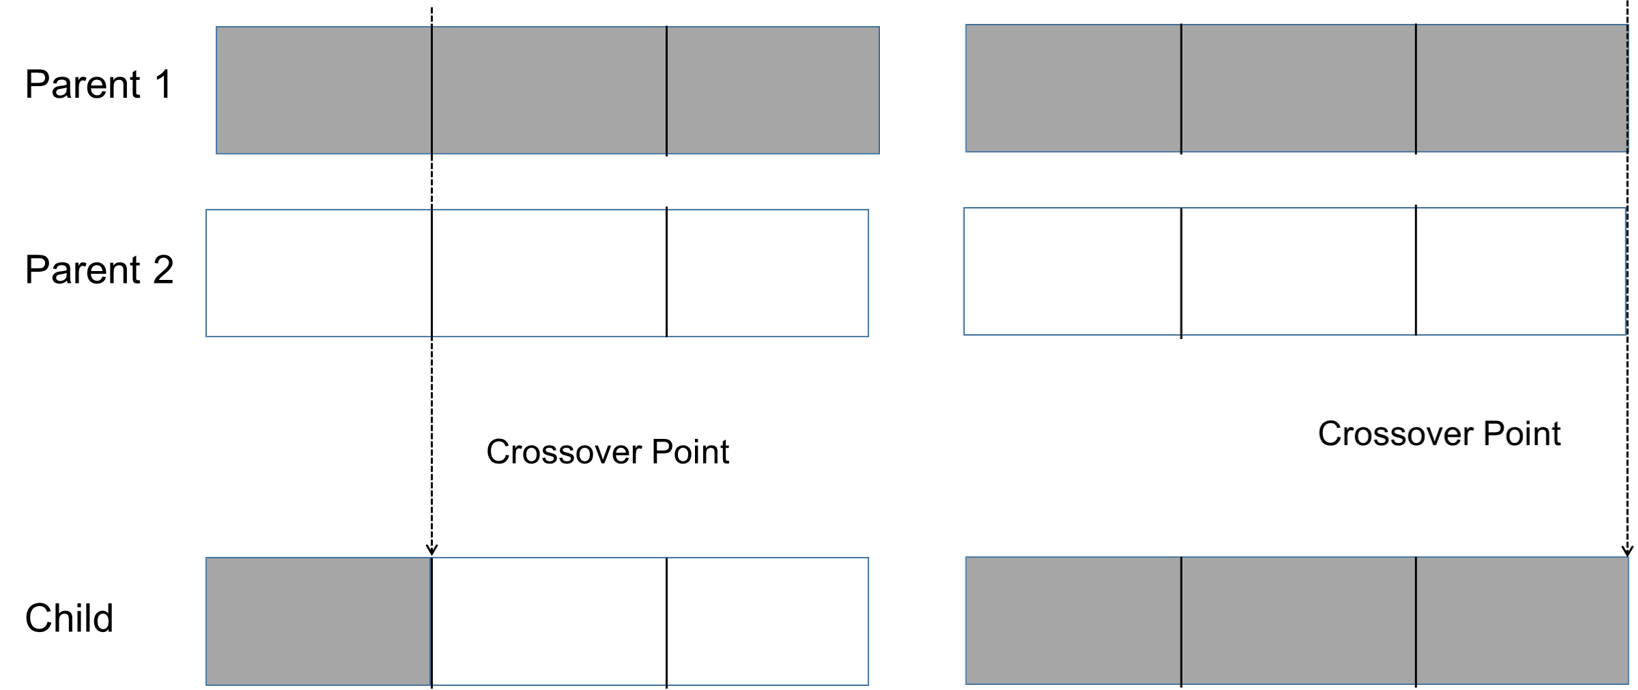
\includegraphics[width=0.45\textwidth]{crossover.png}
            	\caption{Examples of children resulting from crossover between parents.}
            	\label{fig:crossover}
            \end{figure}
        }
    \end{itemize}

	The composition of the next generation, i.e. the percentage of each type of reproduction, is another hyperparameter for this algorithm.
}
\end{enumerate}

\subsection{Hyperparameters}

There are 5 hyperparameters that affect the performance of the gentic algorithm, in terms of speed as well as optimality. The most suitable values for these are determined through trial and error, after running the genetic algorithm multiple times with different values and seeing the trends. The hyperparameters are:

\begin{itemize}
    \item The population size, i.e. number of agents: the time taken is directly proportional to this.
    \item Default weights: this affects how quickly the algorithm can converge to give players with good fitness measures.
    \item Random offset: similar to above, how much the player can be mutated affects the diversity of the population and convergence.	
    \item Number of game rounds: time taken is directly proportional to this.
    \item Composition of new generation: this affects the diversity of players seen 
\end{itemize}


\section{Results}
We came up with a poker agent that can play poker against other agents with different strategies and win or come really close to winning the bigger pot of money. Our agent has a high chance of winning short 100-round games. If there is one thing we would like to explore further if we had the time would be non-linear sum of the heuristics as we think that perhaps a linear sum was perhaps a contributing factor to our agent's bad performance against some strategies.

Additionally, out of 20 sets of 500-round games with {\tt RaisedPlayer}, it won in 16 of them, and 11 of the won games were completely won before the 500 rounds ended. 

\section{Discussion}
During the implementation of the agent, we realised that the runtime was much greater than the recommended 200ms. Upon delving deeper, we found that the game tree has about 40-80 terminal nodes to evaluate heuristics for. And the Monte Carlo simulations method provided by the pypoker engine only to see that running 100 simulations for each node lead to an total overhead of about 400-800ms. There is a trade-off between the number of nodes that we evaluate heuristics for and the number of simulations of Monte Carlo we ran to calculate strength of the Agent's hand. Either way there is a overall decrease in accuracy that we have to take into consideration.

Secondly, the Genetic Algorithm's fitness function method can also be ameliorated. We noticed that the max fitness always lies in the range 0.45 to 0.55 , however it should ideally increase. We suspect it could be because
\begin{itemize}
    \item The heuristics are not normalised and so the weights determined arent scaled to the usual range boundaries of the heuristic values. 
    \item The number of rounds played for fitness (~30), population size (maximum 50) and number of generations (maximum 40) might not be high enough to come up with the most optimal fitness value. 
    \item The fitness function computes a value based on how much money the agent has compared to its opponent (done twice). This may not be the most optimal comparison across all players as compared to a single-player-based heuristic or a round-robin contest.
\end{itemize}

\subsection{Calculating the win rate}

{\bf Alternatives rejected}

\begin{itemize}
    \item TwoPlusTwo Evaluator
    Given our bot’s hole cards and available community cards, return the winrate of the current hand.
    The TwoPlusTwo Evaluator only returns the win rate given the 5/6/7 cards and does not consider the number of players in the match.
    
    \item Monte Carlo simulations
    Using built in function {\tt estimate\_hole\_card\_win\_rate}
    The Monte Carlo simulations provided by the PokerEngine turned out to be too time consuming to do real-time, resulting in numerous TimeOut Exceptions.
\end{itemize} 

\appendix
%% The file named.bst is a bibliography style file for BibTeX 0.99c
\bibliographystyle{named}
\bibliography{ijcai18}

[Denis Richard Papp, 1998] Dealing with imperfect information in poker. Retrieved from http://poker.cs.ualberta.ca/publications/papp.msc.pdf

[Anu Kapadia (n.d.)] Retrieved from https://www.cs.indiana.edu/~kapadia/nofoldem/2\_wins.stats

% https://pdfs.semanticscholar.org/1071/c0f275e5412825d46558e35267a8e03d2b2c.pdf

\end{document}

